\documentclass[a4paper,11pt]{article}

%=========================
% Les styles
%=========================
\usepackage{style-esi/french}	% Francise LaTeX
\usepackage{style-esi/td}
\usepackage{style-esi/licence}	% Affiche une licence dans le document
\usepackage{style-esi/exercice}
\usepackage{style-esi/exemple}
\usepackage{style-esi/listing}
\usepackage{style-esi/tutoriel}
%\marginsectiontrue
\usepackage{booktabs}
\usepackage{pifont} 
%\usepackage{tabularx} 
%\usepackage{multicol}
%\usepackage{multirow}
\usepackage{longtable}
%\usepackage{array}

\definecolor{verylightgray}{rgb}{0.98,0.98,0.98}

\date{2018 -- 2019}
\siglecours{DEV1}
\libellecours{Laboratoires d'environnement}
\libelledocument{TD 6 -- Packages}
\sigleprof{}



\begin{document}

\entete
\titre
\ccbysa{esi-dev1-list@he2b.be}
\lastedit


	%===================
	%  Contenu
	%====================
	\begin{tcolorbox}[blanker,
	before skip=10mm,after skip=10mm,
	borderline west={1mm}{-4mm}{lightgray},
	title=Objectifs, coltitle=black, fonttitle=\sffamily\bfseries\large]
	Dans ce TD, vous allez voir comment organiser vos classes en packages, o\`u les placer et comment les retrouver.
	\end{tcolorbox}
	
	\tableofcontents

	\newpage


%%%%%%%%%%%%%%%%%%%%%%%%%%%%%%%%%%%%%%%%%%%%%%%%%%%%%%%%%%%%%%%%%%%%%%%%%%%%%%%%%%%%%	   
\section{TD6 - Packages}
%%%%%%%%%%%%%%%%%%%%%%%%%%%%%%%%%%%%%%%%%%%%%%%%%%%%%%%%%%%%%%%%%%%%%%%%%%%%%%%%%%%%%
	 \begin{consigne}
	 	\begin{itemize}
			%\item Ce TD est accompagn\'e d'exercices \`a faire \textbf{avant} de venir au laboratoire.
			\item Tout ce que vous allez \'ecrire ici doit se trouver dans un dossier \verb@td6@.
		\end{itemize}				
	\end{consigne}
	
%%%%%%%%%%%%%%%%%%%%%%%	
	\subsection{Demande conviviale de nombres}
%%%%%%%%%%%%%%%%%%%%%%%%
		Rendons les saisies plus conviviales.
			
            \par
        
		\begin{enumerate}
				
			\item Dans une classe \verb@Util@, ajoutez une m\'ethode 
				\verb@int demanderEntier@ \verb@(String msg)@
				qui affiche un message et demande un entier.
				L'entier demand\'e doit apparaitre \`a la suite du message
				et pas \`a la ligne.
			
			\item Afin de tester votre m\'ethode, \'ecrivez une m\'ethode principale qui demande 
				deux entiers et en affiche la somme.
			
		\end{enumerate}
				
		Vous avez probablement envie d'y mettre des couleurs ; par exemple que chaque message d'invite soit en vert.
		Malheureusement, vous ne pouvez pas facilement utiliser votre classe \verb@Color@ car elle est dans un autre dossier.
		La seule solution que vous pouvez envisager, pour le moment, est de prendre une copie du \verb@.class@ ou une copie de votre source
		et de le recompiler ; ce n'est \'evidemment pas pratique...
			
            \par
        
			
		Pour pouvoir utiliser une classe qui se trouve ailleurs, il faut la ranger dans un \textit{package}.
		C'est ce que nous allons vous expliquer \`a pr\'esent.
		
			
            \par
	
%%%%%%%%%%%%%%%%%%%%%%%%%%%%%%%%%%%%%%%%%%%%%%%%%%%%%%%%%%%%%%%%%%%%%%%%%%%%%%%%%%			
 	 \subsection{Introduction aux packages}
%%%%%%%%%%%%%%%%%%%%%%%%%%%%%%%%%%%%%%%%%%%%%%%%%%%%%%%%%%%%%%%%%%%%%%%%%%%%%%%%%%		
		Vous \^etes capables d'utiliser une classe qui a \'et\'e plac\'ee dans un package standard 
		(comme \verb@java.util.Scanner@). Nous allons \`a pr\'esent vous montrer
		comment placer vos propres classes dans des packages et les utiliser.
			
            \par
        
			
		\subparagraph{Le nom d'un package} 
		
				\textcolor{white}{.} 
				
				Un nom de package doit \^etre choisi de telle sorte \`a repr\'esenter l'organisation \`a laquelle elle
				appartient et le projet associ\'e ou le type de classe. Il ne faut pas se baser sur l'endroit o\`u sont plac\'es 
				les fichiers sources.
			
            \par
        
				Pour \textbf{votre} code, nous vous recommandons de rassembler vos classes par package reprenant votre login et le TD.
				Exemple : \verb|g32010.td6|
			
            \par
        
			
		\subparagraph{Associer une classe \`a un package} 
		
					\textcolor{white}{.} 
				
           			L'appartenance d'une classe \`a un package d\'etermin\'e est n\'ecessaire \`a la compilation. 
				D\`es lors vous devrez ajouter comme \textbf{premi\`ere instruction du source} 
				(c-\`a-d avant m\^eme l'instruction \verb|public class NomClasse|) :
			
            \par
        				\begin{Code}{java}
					package g32010.td6;
				\end{Code}
			
		\subparagraph{Nom complet d'une classe} 
		
					\textcolor{white}{.} 
				
          			Le nom \textbf{qualifi\'e} d'une classe (on dit aussi \textbf{nom complet})
				est obtenu en accolant le nom de la classe au nom du package ; on obtient ainsi un nom unique pour cette classe.
				C'est ce nom qu'il faudra utiliser pour \textbf{ex\'ecuter} la classe.
			
            \par
        
				Par exemple, le nom complet de la classe \verb@Color@ dont le package est \verb|esi.util|
				est \verb|esi.util.Color|. 
			
            \par
        		\begin{Exercice}{}
				Donnez le nom complet de la classe \verb@SurfaceTriangle@ dont le package est 
				\verb@g32010.td6@ : 
				\par
				\fcolorbox{gray}{verylightgray}{
					\begin{minipage}[c][1cm][c]{\textwidth}\textcolor{verylightgray}{X}\end{minipage}
				}%\par\medskip
		\end{Exercice}	
		
		\subparagraph{Package et dossiers} 
		
				\textcolor{white}{.} 
									
				Alors qu'on peut placer ses fichiers sources (les .java) o\`u on veut, ce n'est pas le cas pour les fichiers
				compil\'es (les .class) d\`es lors qu'on joue avec des packages. Ils devront \^etre plac\'es \`a un endroit bien pr\'ecis
				pour que le compilateur et la machine virtuelle puissent les retrouver.
			
            \par
        			
				La notion de package est li\'ee \`a celle de r\'epertoire (et m\^eme d'arborescence de r\'epertoires).
				Ainsi le package \verb|td.td6| sera associ\'e aux dossiers \verb@td/td6@
				(un dossier \verb|td6| dans un dossier \verb|td|).Tout comme une classe appartient \`a un package,
				la version compil\'ee de la classe devra se trouver dans les dossiers correspondant au package.
			
            \par
        
			
		\begin{Exemple}{}
			Si \verb|Color| a pour package \verb|esi.util|, le fichier \verb@Color.class@
				devra se trouver dans le r\'epertoire associ\'e \verb@esi/util@.
		\end{Exemple}
			
            \par
        
			
		\begin{Exercice}{}
       				Examinez le contenu du dossier \verb@esi/util@
				qui se trouve dans \verb@/eCours/Java@.
		\end{Exercice}
			
            \par
        
			
		\begin{Exercice}{} 
       			Donnez la suite de r\'epertoires dans lesquels \textbf{doit} certainement se trouver la classe \verb|SurfaceTriangle|
			dont le package est  \verb|g32010.tds.td6| :
			\par
			\fcolorbox{gray}{verylightgray}{
					\begin{minipage}[c][1cm][c]{\textwidth}\textcolor{verylightgray}{X}\end{minipage}
				}
		\end{Exercice}	
			
			
%%%%%%%%%%%%%%%%%%%%%%%%%%%%%%%%%%%%%%%%%%%%%%%%%%%%%%%%%%%%%%%%%%%%%%%%			
	\subsection{Utiliser le package d'un autre}
%%%%%%%%%%%%%%%%%%%%%%%%%%%%%%%%%%%%%%%%%%%%%%%%%%%%%%%%%%%%%%%%%%%%%%%%
		Lors du pr\'ec\'edent TD, vous avez pris une copie de la classe \verb@Color@
		et vous l'avez compil\'ee. Nous avons aussi fait ce travail en pla\c cant la classe dans le package
		\verb@esi.util@. Voyons voir comment l'utiliser.			
		
            \par
        
			
		\begin{Tutoriel}{Exp\'erience} 
   			\begin{steps}
				
				\item La classe poss\`ede une m\'ethode principale. Tentez de l'ex\'ecuter via la commande
					\begin{Console}
						java Color
					\end{Console}
					
					\par
				
					Ca ne fonctionne pas. Pourquoi ?
			
				\item  Mais bien s\^ur ; on a dit qu'il fallait utiliser le nom complet de la classe.
					Tentez la commande :
					\begin{Console} 
						java esi.util.Color
					\end{Console}
					\par
				
					Zut ! Ca ne fonctionne toujours pas. Pourquoi ?
			
					 Parce que Java ne sait pas o\`u trouver la classe
					et il est hors de question de chercher dans tout le syst\`eme de fichier.
				
            				\par
        
					O\`u est-elle d'ailleurs, cette classe ?
				
            				\par
        
					\item Pour le savoir, lan\c cez la commande :
						\begin{Console} 
							find /eCours/java -name Color.class
						\end{Console}
					Vous devriez voir que la classe se trouve exactement ici :\par
					 \verb@/eCours/java/esi/util/Color.class@
            				\par
        
					\item On va indiquer \`a Java o\`u chercher.
						Entrez la commande
						\begin{Console}
							java -cp /eCours/java esi.util.Color
						\end{Console}
				
					Cette fois-ci \c ca fonctionne !
			
			\end{steps}
		\end{Tutoriel}		
			L'option \verb@cp@ (une abr\'eviation pour \verb@classpath@) indique le (ou les) endroit(s) o\`u chercher les classes.
		
           	 \par
        			\textbf{Important ! } on ne donne pas le dossier o\`u se trouve le \textit{.class}
			mais le dossier o\`u il va pouvoir trouver la hi\'erarchie de dossiers li\'ee au package.
			Finalement, le fichier se trouve \`a un endroit qui est la \textit{concat\'enation} de l'option \textit{cp}
			et du package.
		
            \par

%%%%%%%%%%%%%%%%%%%%%%%%%%%%%%%		
	 \subsection{Utiliser ses propres packages}
%%%%%%%%%%%%%%%%%%%%%%%%%%%%%%%			
		\`A pr\'esent, nous allons voir comment vous pouvez placer vos propres classes dans un package.
		
            \par
        
			
		\begin{Tutoriel}{Exp\'erience} 
         		\begin{steps}
				\item Prenez une copie de la classe \verb@Color@.	
			
				\item Ajoutez comme premi\`ere ligne :
					\begin{Code}{java}
						package g12345.util;
					\end{Code}
				\item Compilez-la : 
					\begin{Console}
						javac Color.java
					\end{Console}
				\item Ex\'ecutez-la : 
					\begin{Console}
						java -cp . g12345.util.Color
					\end{Console}
				\par
				
					\c Ca ne fonctionne pas ! Pourquoi ?
			
				 Qu'on est b\^ete ! Java cherche le fichier dans une hi\'erarchie
				de dossiers correspondant au package. Ici, il cherche le fichier
				\verb@g12345/util/Color.class@
					
				\item D\'epla\c cons le fichier au bon endroit.
				\par
					\begin{Console}
						mkdir -p g12345/util
						mv Color.class g12345/util
					\end{Console}
				\item Re-tentons : 
					\begin{Console}
						java -cp . g12345.util.Color
					\end{Console}
				\par
				
				\c Ca fonctionne !
			
					\end{steps}
				\end{Tutoriel}
			
		\subparagraph{J'ai oubli\'e l'option '-cp' et \c ca fonctionne quand m\^eme !?} 
		
					\textcolor{white}{.} \par
				
          		En effet, sur linux1, et nous verrons pourquoi, si on ne lui  dit pas o\`u chercher, 
			il cherche dans le dossier courant.
		
            		\par
        
			
		\subparagraph{L'option -d} 
		
					\textcolor{white}{.} \par

			Ce serait p\'enible de devoir d\'eplacer, apr\`es chaque compilation,
			la classe au bon endroit. Heureusement, le compilateur propose une option
			qui place directement le fichier g\'en\'er\'e au bon endroit.
		
            		\par
        
			La commande
		
            		\par
       			 \begin{Console}
				javac -d chemin Fichier.java
			\end{Console}
			Compile le fichier donn\'e et place le r\'esultat dans une hi\'erarchie de dossiers
			qui correspond au package \`a partir du chemin donn\'e.
		
           		 \par
        
			
		\begin{Exemple}{} 
			Pour la classe couleur, on aurait pu compiler simplement avec la commande :
				\begin{Console}
					javac -d . Color.java
				\end{Console}
			pour indiquer de cr\'eer le r\'esultat dans le dossier \verb@./g12345/util/@.
		\end{Exemple}
		
            \par
%%%%%%%%%%%%%%%%%%%%%%%%%%%%%%%%%%%%%%%%%%%%%%%%%%%%%%%%%%%%%%%%%%%%%%%%%%
        \subsection{La variable CLASSPATH}
%%%%%%%%%%%%%%%%%%%%%%%%%%%%%%%%%%%%%%%%%%%%%%%%%%%%%%%%%%%%%%%%%%%%%%%%%%%
		Sp\'ecifier \`a chaque fois, l'option \verb@cp@ est p\'enible.
		Ce serait bien de pouvoir lui dire une fois pour toutes o\`u chercher.
		C'est exactement le r\^ole de la variable d'environnement \verb@CLASSPATH@.
			
            	\par
        
		\begin{colxbox}
				La variable \verb@CLASSPATH@ contient une liste de dossiers o\`u chercher les
				classes. Chaque dossier est s\'epar\'e par "\verb@:@".
		\end{colxbox}	
			

		Pour la manipuler, la proc\'edure est la m\^eme que pour les autres variables d'environnement
		(comme \verb@PS1@ que vous avez d\'ej\`a vu).
			
           	 \par
        
		\begin{itemize}
				
			\item Pour voir son contenu : \verb@echo $CLASSPATH@
			\item Pour changer son contenu : \verb@CLASSPATH=valeur@
			\item Pour ajouter un dossier \`a son contenu : 
					\verb@CLASSPATH=$CLASSPATH:valeur@
			\item Si elle est d\'efinie pour la premi\`ere fois : 
					\verb@export CLASSPATH@
			\item Si la modification doit \^etre permanente, vous pouvez placer la commande dans le fichier
					\verb@.bashrc@
		\end{itemize}
				
			
		\begin{Exercice}{} 
			Affichez le contenu actuel de la variable \verb@CLASSPATH@.
			Que signifie le "." ?
		\end{Exercice}
			
            \par
        
			
		\begin{Exercice}{}
			Sachant que la classe \verb|SurfaceTriangle| se trouve dans \verb@/home/g32010/tds/td6@ 
			et qu'on retrouve \verb@/home@ dans la variable \verb@CLASSPATH@, 
			donnez l'instruction \verb|package| correspondant \`a la situation :
			\begin{colxbox}
				   package                            
			\end{colxbox}
		\end{Exercice}
			
		\begin{Exercice}{} 
				Supposons que la classe \verb|Exercice1| a pour package \verb|esi.lg1.exemples|
				et qu'elle a comme chemin \verb@/eCours/java/be/heb/esi/lg1/exemples/Exercice1.class@, 
				donnez la hi\'erarchie de r\'epertoires \`a ajouter au \verb@CLASSPATH@.
				\begin{colxbox}	
				CLASSPATH=\$CLASSPATH: 
				\end{colxbox}
		\end{Exercice}
			
		\begin{Exercice}{} 
			Faites ce qu'il faut pour pouvoir ex\'ecuter \textbf{notre} classe \verb@Color@
			(package \verb@esi.util@) sans utiliser l'option \verb@-cp@.
		\end{Exercice}
			
           	 \par
%%%%%%%%%%%%%%%%%%%%%%%%%%%%%%%%%%		
	 \subsection{Organiser ses fichiers}
%%%%%%%%%%%%%%%%%%%%%%%%%%%%%%%%%%
		R\'esumons ce que  nous avons d\'ej\`a vu.
			
            	\par
        
		\begin{itemize}
				
			\item un package est un regroupement de classes ;
				
			\item pour cr\'eer un tel package, il suffit de commencer les 
				\textbf{fichiers sources} contenant les classes \`a regrouper
				par l'instruction \verb@package@ suivi du nom que l'on d\'esire donner au package ;
				
			\item les \textbf{fichiers classes} doivent se trouver dans l'arborescence de r\'epertoires 
					donn\'ee par le package.
				
			\item Cette arborescence doit commencer dans un dossier
				repris dans le CLASSPATH.
				
		\end{itemize}
				
		Mais, concr\'etement, quel dossier choisir pour placer les classes ?
		Il existe plusieurs fa\c cons de s'organiser ; on va vous en pr\'esenter deux. 
			
            \par
        
			
		\subparagraph{Sans package.} 
		
					\textcolor{white}{.} \par
				
			Avant de vous présenter ces deux fa\c ons, r\'esumons, d'abord, ce que vous faisiez jusqu'\`a pr\'esent sans package.
			Avec cette approche, le source et la classe se trouvent dans un m\^eme dossier, quelconque.
			
            \par
        
			\begin{enumerate}
				
				\item On se place o\`u on veut.
				
				\item On \'edite le source : 
					\begin{Console}
						nano Test.java
					\end{Console}
				\item On compile : 
					\begin{Console}
						javac Test.java
					\end{Console}
				\item On ex\'ecute :
					 \begin{Console}
					 	java Test
					\end{Console}
			\end{enumerate}
				
			
			\begin{Tutoriel}{1\`ere proposition : pour transporter vos sources et classes rapidement.} 
				Dans cette approche, les sources sont s\'epar\'es des classes mais sont dans un dossier commun.
			
            		\par
       			 	\begin{figure}[hbt]
				    	\begin{center}
						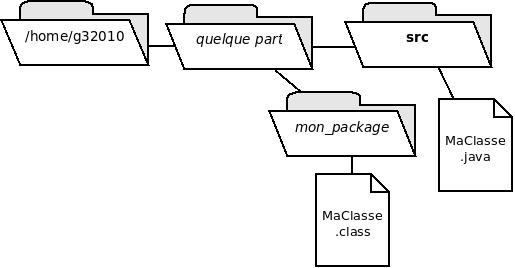
\includegraphics[width=0.6\linewidth,height=0.8\textheight,keepaspectratio=true]{image/approche4.jpeg}
					\end{center}
                
                   			 \caption[Illustration de la 1\`ere approche]{Illustration de la 1\`ere approche}
               			 \end{figure}
                    
				\begin{steps}
				
					\item On v\'erifie que le CLASSPATH contient bien le 
						dossier courant (sur linux1, c'est le cas).
				
					\item On se place quelque part.
				
					\item On cr\'ee un dossier pour les sources : 
						\begin{Console}
							mkdir src
						\end{Console}
					\item On \'edite le source dans le dossier d\'edi\'e : 
						\begin{Console}
							nano src/Test.java
						\end{Console}
				
						en prenant soin de commencer le fichier par un package qui a du sens
						(par exemple : \verb@g12345.td6@).
				
					\item On compile en demandant \`a cr\'eer la classe \`a partir
						du dossier courant : 
						\begin{Console}
							javac -d . src/Test.java
						\end{Console}
					\item On ex\'ecute : 
						\begin{Console}
							java g12345.td6.Test
						\end{Console}
				\end{steps}
				
			\end{Tutoriel}	
		\begin{Exercice}{}
				Dans un sous-dossier du td6 (par exemple : td6/cas1), faites une copie de votre programme 
				\verb@Hello.java@ d\'evelopp\'e au td3 et placez-le dans un package en suivant l'approche ci-dessus.
				Quelle est la commande \`a utiliser pour compiler ? Et pour ex\'ecuter ?
		\end{Exercice}
			
           	 \par
        
			\fcolorbox{gray}{verylightgray}{
				\begin{minipage}[c][2cm][c]{\textwidth}\textcolor{verylightgray}{X}\end{minipage}
				}\par\medskip
			
		\subparagraph{Remarques} 
		
			\textcolor{white}{.} \par
					
			\begin{itemize}
				
				\item Il existe de nombreuses variantes. Par exemple, les sources dans le dossier
					"src" et les classes dans le dossier "classes" ou encore les classes dans le dossier "classes"
					mais les sources directement dans le dossier courant. 
				
				\item Cette approche permet de facilement copier tous les sources et les classes associ\'ees
				
				\item Par contre, les classes ne peuvent pas s'ex\'ecuter
					de partout.
			 	
			\end{itemize}
				
			
		\begin{Tutoriel}{2\`eme proposition : toutes les classes sont regroup\'ees dans le m\^eme dossier (\char`\~/classes).} 
			Dans cette approche, toutes les classes de tous vos projets sont plac\'ees dans un dossier commun
			(par exemple : \verb@~/classes@)
			
           		 \par
       			 \begin{figure}[hbt]
				 \begin{center}
					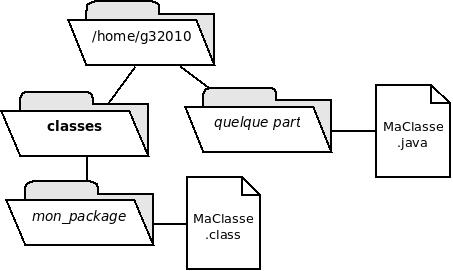
\includegraphics[width=0.6\linewidth,height=0.8\textheight,keepaspectratio=true]{image/approche3.jpeg}
				\end{center}
                
                   		 \caption[Illustration de la 2\`eme approche]{Illustration de la 2\`eme approche}
               		 \end{figure}
                    
			\begin{steps}
				
				\item Il faut s'assurer que le CLASSPATH contienne le dossier \verb@~/classes@.
					Si ce n'est pas le cas, il faut le d\'efinir (une fois pour toutes
					dans le fichier de configuration du bash) : \verb@CLASSPATH=$CLASSPATH:~/classes@.					
				
				\item On se place quelque part.
				
				\item On \'edite le source directement dans le dossier courant : 
					\begin{Console}
						nano Test.java
					\end{Console}
					en prenant soin de commencer le fichier par un package qui a du sens
					(par exemple : \verb@g12345.td6@).
				
				\item On compile en demandant \`a cr\'eer la classe dans
					le dossier global d\'edi\'e :
					\begin{Console}
						javac -d ~/classes Test.java
					\end{Console}
				\item On ex\'ecute : 
					\begin{Console}
						java g12345.td6.Test
					\end{Console}
			\end{steps}
		\end{Tutoriel}		
			
		\begin{Exercice}{}
				Il s'agit du m\^eme exercice que pour la premi\`ere approche.
				Dans un autre sous-dossier du td6 (par exemple : td6/cas2),
				faites une copie de votre programme \verb@Hello.java@ d\'evelopp\'e au td3
				et placez-le dans un package en suivant l'approche ci-dessus.
				Quelle est la commande \`a utiliser pour compiler ?
				Et pour ex\'ecuter ?
		\end{Exercice}
			
            \par
        
		\fcolorbox{gray}{verylightgray}{
			\begin{minipage}[c][2cm][c]{\textwidth}\textcolor{verylightgray}{X}\end{minipage}
		}\par\medskip 
				
	\begin{Exercice}{Netbeans}
	Vous venez de voir 2 façons d'organiser votre projet (emplacement pour les sources et les classes). 
		\begin{itemize}
			\item Quel est le choix exact fait par Netbeans ? 
			\item Que voyez-vous comme avantages/inconvénients ?
		\end{itemize}
	\end{Exercice}		
\end{document}
			